% Topographic Mapping -- Guided Notes
% Compile twice: student version as-is; answer key with \printanswers uncommented.
\documentclass[11pt,addpoints]{exam}

\ifdefined\KEYBUILD\printanswers\fi  % key build: pdflatex "\def\KEYBUILD{}% Topographic Mapping -- Guided Notes
% Compile twice: student version as-is; answer key with \printanswers uncommented.
\documentclass[11pt,addpoints]{exam}

\ifdefined\KEYBUILD\printanswers\fi  % key build: pdflatex "\def\KEYBUILD{}% Topographic Mapping -- Guided Notes
% Compile twice: student version as-is; answer key with \printanswers uncommented.
\documentclass[11pt,addpoints]{exam}

\ifdefined\KEYBUILD\printanswers\fi  % key build: pdflatex "\def\KEYBUILD{}% Topographic Mapping -- Guided Notes
% Compile twice: student version as-is; answer key with \printanswers uncommented.
\documentclass[11pt,addpoints]{exam}

\ifdefined\KEYBUILD\printanswers\fi  % key build: pdflatex "\def\KEYBUILD{}\input{topographic-mapping-guided-notes.tex}"
%\printanswers  % <-- or just uncomment this line for the answer key

\usepackage[margin=0.85in,top=1.0in,headsep=0.25in]{geometry}
\usepackage{graphicx}
\usepackage{amsmath}
\usepackage{xcolor}
\usepackage{tikz}
\usepackage{enumitem}
\usepackage{multicol}
\usepackage{tcolorbox}

\definecolor{keyblue}{RGB}{0,70,190}
\definecolor{accent}{RGB}{29,107,132}
\definecolor{shade}{RGB}{234,243,246}

\setlength{\parindent}{0pt}
\setlength{\parskip}{4pt}

% ---------- fill-in-the-blank macro ----------
% \blk{answer} or \blk[width]{answer}
\newcommand{\blk}[2][3.2cm]{%
  \ifprintanswers
    \underline{\textcolor{keyblue}{\textbf{#2}}}%
  \else
    \underline{\hspace{#1}}%
  \fi}

% teacher-only note
\newcommand{\teachernote}[1]{\ifprintanswers\par\textcolor{accent}{\textit{Teacher note: #1}}\par\fi}

\newcommand{\term}[1]{\textbf{\textcolor{accent}{#1}}}

\newtcolorbox{callout}{colback=shade,colframe=accent,boxrule=0.8pt,left=8pt,right=8pt,top=6pt,bottom=6pt,arc=2pt}

% ---------- header ----------
\pagestyle{headandfoot}
\header{\textbf{Topographic Mapping --- Guided Notes}}{}{%
  \ifprintanswers\textcolor{keyblue}{\textbf{ANSWER KEY}}\else Name: \underline{\hspace{4cm}}\fi}
\footer{}{Page \thepage\ of \numpages}{}
\runningheadrule
\runningfootrule

\begin{document}

\ifprintanswers\else
{\small Period: \underline{\hspace{2cm}} \hfill Date: \underline{\hspace{3.5cm}}}
\vspace{6pt}
\fi

\begin{callout}
\textbf{Objective:} Use isolines to represent field data, construct a topographic profile from a contour map, and calculate gradient using the ESRT equation.
\end{callout}

%==========================================================
\section*{1. Mapping the Earth: Terms}

A \term{field} is any region of space that has a measurable value of a given quantity at \blk[3cm]{every point}.

An \term{isoline} is a line that connects points of \blk[3.5cm]{equal value}.

\vspace{4pt}
Fill in the table:

\begin{center}
\renewcommand{\arraystretch}{1.7}
\begin{tabular}{|p{3.2cm}|p{5.5cm}|p{4.5cm}|}
\hline
\textbf{Type of isoline} & \textbf{Connects points of equal\dots} & \textbf{Where you see it} \\ \hline
Isotherm & \blk[3.5cm]{temperature} & Weather map \\ \hline
Isobar & \blk[3.5cm]{pressure} & Weather map \\ \hline
Contour line & \blk[3.5cm]{elevation} & Topographic map \\ \hline
\end{tabular}
\end{center}

\teachernote{Point out the prefix \textit{iso-} = equal. Students who learn the prefix can decode any isoline question on the Regents exam, including ones they have never seen (isoseismal, isohyet).}

\vspace{4pt}
A topographic map shows a \blk[2.5cm]{3-D} landscape on a \blk[2.5cm]{2-D} sheet of paper. Each contour line traces one elevation all the way around the landform.

\begin{center}
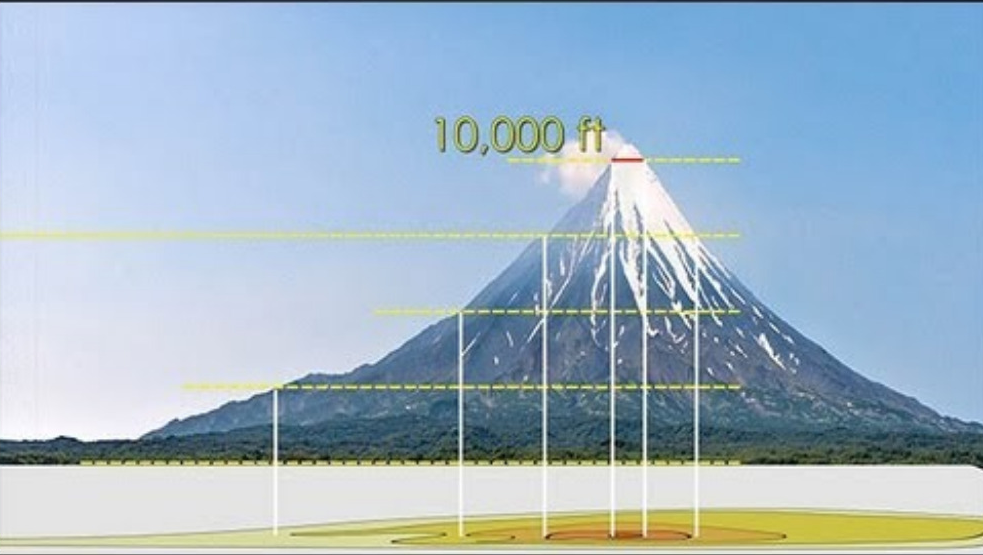
\includegraphics[width=0.62\textwidth]{images/mountain-contours.png}
\end{center}

%==========================================================
\section*{2. How to Draw an Isoline}

\begin{enumerate}[leftmargin=*,itemsep=6pt]
  \item Connect dots of \blk[3cm]{equal value}, using the interval stated in the directions.
  \item Where the exact number is not printed, \blk[2.5cm]{estimate} where it would fall between a point of higher value and a point of lower value.
  \item Bring every isoline all the way to the \blk[3cm]{edge of the field}.
\end{enumerate}

\textbf{Rules isolines never break:}

\begin{multicols}{2}
\begin{itemize}[leftmargin=*,itemsep=4pt]
  \item Isolines never \blk[2cm]{cross} each other.
  \item Isolines never split or branch.
  \item Isolines close into loops or run off the map edge.
  \item Values change \textbf{in order} --- no skipping.
  \item Lines close together $=$ value changing \blk[2cm]{quickly}.
  \item Lines far apart $=$ value changing \blk[2cm]{slowly}.
\end{itemize}
\end{multicols}

\subsection*{Practice: elevation field (contour interval = 10 ft)}

Draw contour lines at 40, 50, 60, 70, and 80 feet. Label each line and carry it to the edge of the box.

\begin{center}
\begin{tikzpicture}[x=2.0cm,y=1.5cm]
  \def\vals{
    {42,48,55,61,58,51},
    {47,56,68,72,65,55},
    {52,63,78,85,71,58},
    {49,58,70,76,66,54},
    {44,51,59,63,57,48},
    {38,43,48,52,47,41}}
  \foreach \row [count=\r from 0] in \vals {
    \foreach \v [count=\c from 0] in \row {
      \fill (\c,-\r) circle (1.3pt);
      \node[anchor=south west,font=\small,inner sep=1.5pt] at (\c,-\r) {\v};
    }
  }
  \draw[thick] (-0.35,0.6) rectangle (5.55,-7.85);
  \node[anchor=north west,font=\small\itshape] at (-0.35,-7.95) {Elevation (feet)};
\end{tikzpicture}
\end{center}

\teachernote{The 80-ft line is a small closed loop around the 85 value near the center; the 40-ft line only appears along the bottom edge. Watch for students who connect \textit{nearest dots} instead of \textit{equal values} --- have them label the two dots they are interpolating between before they draw.}

%==========================================================
\newpage
\section*{3. Map Scale and Direction}

\term{Map scale:} a ratio of the distance between two places on a map and the \blk[4cm]{actual distance} on Earth's surface.

\term{Cardinal directions:} \blk[1.8cm]{north}, \blk[1.8cm]{south}, \blk[1.8cm]{east}, \blk[1.8cm]{west}, and any combination of these (NE, SW, \dots).

\begin{center}
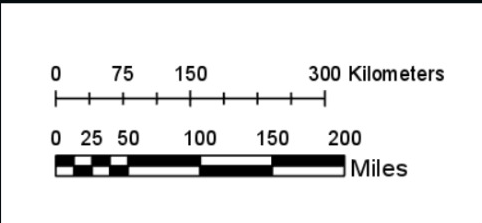
\includegraphics[width=0.42\textwidth]{images/map-scale.png}
\hspace{0.5cm}
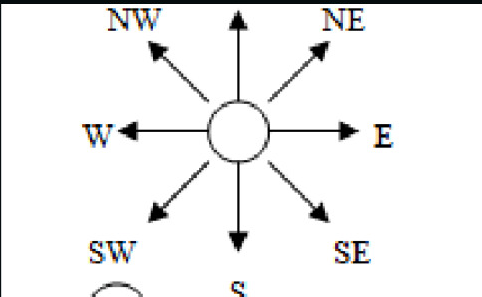
\includegraphics[width=0.26\textwidth]{images/compass-rose.png}
\end{center}

%==========================================================
\section*{4. Constructing a Profile}

A \term{profile} is a \blk[3.5cm]{side view} of the land along a line drawn on the map.

\begin{enumerate}[leftmargin=*,itemsep=6pt]
  \item Line the edge of a piece of \blk[3cm]{scrap paper} up with the two points on your map.
  \item Mark the two endpoints, plus every \blk[3cm]{contour line} that falls between them.
  \item Write the \blk[2cm]{value} of every mark.
  \item Line the paper edge up with the \blk[2cm]{x-axis} of your graph (first point at the origin) and plot each elevation against the \blk[2cm]{y-axis}.
  \item Connect your points with a \blk[3cm]{smooth curve}.
\end{enumerate}

\begin{callout}
\textbf{Round out the tops of your peaks and the bottoms of your valleys.} The land keeps rising past the last contour line you crossed, so the hilltop is rounded --- not a sharp point. \textbf{Straight lines and sharp peaks receive no credit.}
\end{callout}

\begin{center}
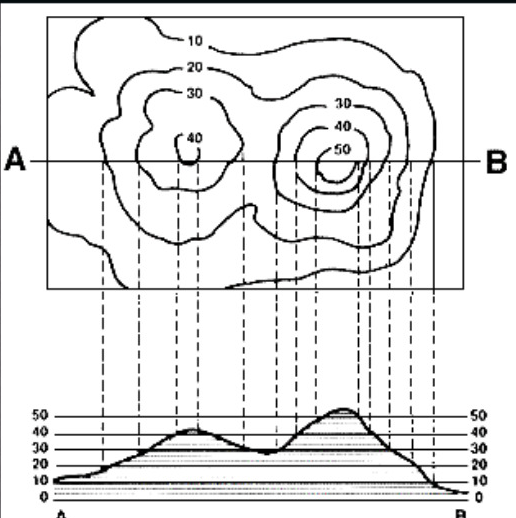
\includegraphics[width=0.38\textwidth]{images/profile-ab.png}
\end{center}

\subsection*{Practice: plot the profile}

Elevations were read along line A--B and recorded below. Plot each point, then connect them with a smooth, rounded curve.

\begin{center}
\small
\begin{tabular}{|c|c|c|c|c|c|c|c|c|c|c|c|}
\hline
\textbf{Point} & A & 2 & 3 & 4 & 5 & 6 & 7 & 8 & 9 & 10 & B \\ \hline
\textbf{Elev. (ft)} & 20 & 30 & 40 & 40 & 30 & 20 & 30 & 40 & 50 & 40 & 30 \\ \hline
\end{tabular}
\end{center}

\begin{center}
\begin{tikzpicture}[x=1.3cm,y=0.09cm]
  \draw[gray!45] (0,0) grid[xstep=1.3cm,ystep=0.09cm] (10,60);
  \foreach \y in {0,10,20,30,40,50,60} {
    \draw[gray!70] (0,\y) -- (10,\y);
    \node[anchor=east,font=\small] at (-0.08,\y) {\y};
  }
  \foreach \x in {0,1,2,3,4,5,6,7,8,9,10} \draw[gray!70] (\x,0) -- (\x,60);
  \draw[thick] (0,0) rectangle (10,60);
  \node[anchor=north,font=\small] at (0,-1) {A};
  \node[anchor=north,font=\small] at (10,-1) {B};
  \foreach \x [count=\i from 2] in {1,2,3,4,5,6,7,8,9} \node[anchor=north,font=\small] at (\x,-1) {\i};
  \node[rotate=90,anchor=south,font=\small] at (-0.75,30) {Elevation (ft)};
  \ifprintanswers
    \draw[keyblue,very thick,smooth]
      plot coordinates {(0,20) (1,30) (2,40) (3,40) (4,30) (5,20) (6,30) (7,40) (8,50) (9,40) (10,30)};
    \foreach \p in {(0,20),(1,30),(2,40),(3,40),(4,30),(5,20),(6,30),(7,40),(8,50),(9,40),(10,30)}
      \fill[keyblue] \p circle (2.2pt);
  \fi
\end{tikzpicture}
\end{center}

\teachernote{The key shows the plotted points connected point-to-point. Students should smooth the curve and round the two hilltops \textit{above} 40 ft and 50 ft respectively, and round the low point near point 6 --- the exact values between marks are unknown, which is the whole reason the curve is drawn smooth.}

%==========================================================
\newpage
\section*{5. Contour Lines and Streams}

\begin{itemize}[leftmargin=*,itemsep=4pt]
  \item Contour lines \blk[2cm]{bend} where they cross a stream.
  \item The bend forms a V that points \blk[2.5cm]{upstream} (uphill).
  \item Water flows \blk[2.5cm]{downhill}, so the stream flows in the \textbf{opposite} direction from the V.
  \item Streams run from \blk[2cm]{high} elevation toward \blk[2cm]{low} elevation.
\end{itemize}

\begin{center}
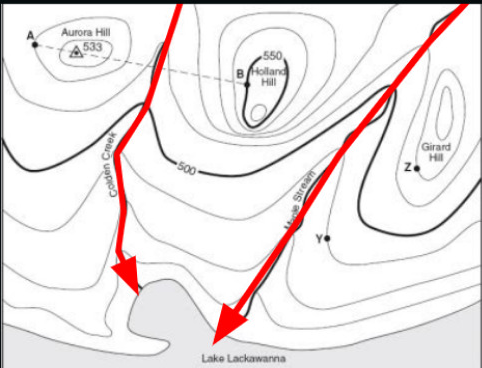
\includegraphics[width=0.60\textwidth]{images/stream-contours.png}
\end{center}

\begin{questions}

\question[2] On the map above, in which compass direction does Coldan Creek flow? Explain how the contour lines tell you.
\ifprintanswers
  \par\textcolor{keyblue}{\textbf{South (toward Lake Lackawanna).} The Vs in the contour lines point north --- upstream --- and the contour values decrease toward the lake, so the water flows south, from high elevation to low.}
\else
  \fillwithlines{0.9in}
\fi

\end{questions}

%==========================================================
\section*{6. Gradient}

Gradient tells you how \blk[2.5cm]{steep} a slope is. The equation is on page \blk[1cm]{1} of the ESRT:

\begin{callout}
\[ \text{Gradient} = \frac{\text{change in field value}}{\text{distance}} \]
\end{callout}

The closer the isolines are together in a given distance, the \blk[2cm]{larger} the gradient.

\textbf{Worked example.} Point A is at 123 feet. Point B is at 20 feet. The points are 2 miles apart.

\[ \text{Gradient} = \frac{123\ \text{ft} - 20\ \text{ft}}{2\ \text{mi}} = \frac{\blk[1.6cm]{103}\ \text{ft}}{2\ \text{mi}} = \blk[2cm]{51.5}\ \text{ft/mi} \]

\begin{center}\textbf{DON'T FORGET UNITS!}\end{center}

\teachernote{Require all three steps every time --- equation, substitution with units, answer with units. Regents rubrics award credit for the setup even when the arithmetic slips.}

\begin{questions}

\question[3] Point A has an elevation of 260 feet. Point B has an elevation of 10 feet. The points are 3 miles apart. Calculate the gradient. Show the equation, your substitution, and the units.
\ifprintanswers
  \par\textcolor{keyblue}{$\text{Gradient} = \dfrac{\text{change in field value}}{\text{distance}} = \dfrac{260\ \text{ft} - 10\ \text{ft}}{3\ \text{mi}} = \dfrac{250\ \text{ft}}{3\ \text{mi}} = \mathbf{83.3\ \text{ft/mi}}$}
\else
  \fillwithlines{1.1in}
\fi

\question[3] A hilltop is 550 meters above sea level. A stream at the base of the hill is 250 meters above sea level. The horizontal distance between them is 1.5 kilometers. Calculate the gradient.
\ifprintanswers
  \par\textcolor{keyblue}{$\dfrac{550\ \text{m} - 250\ \text{m}}{1.5\ \text{km}} = \dfrac{300\ \text{m}}{1.5\ \text{km}} = \mathbf{200\ \text{m/km}}$}
\else
  \fillwithlines{1.1in}
\fi

\question[3] On a weather map, one station reports 82\,$^\circ$F and another reports 58\,$^\circ$F. The stations are 4 kilometers apart. Calculate the temperature gradient between them.
\ifprintanswers
  \par\textcolor{keyblue}{$\dfrac{82\,^\circ\text{F} - 58\,^\circ\text{F}}{4\ \text{km}} = \dfrac{24\,^\circ\text{F}}{4\ \text{km}} = \mathbf{6\,^\circ\text{F/km}}$ --- gradient works on \textit{any} field, not just elevation.}
\else
  \fillwithlines{1.1in}
\fi

\question[2] Two trails climb the same hill. Trail X crosses contour lines that are crowded close together; trail Y crosses contour lines that are widely spaced. Which trail is steeper, and how do you know?
\ifprintanswers
  \par\textcolor{keyblue}{\textbf{Trail X.} Crowded contours mean a large change in elevation over a short distance, which is a large gradient --- a steeper slope.}
\else
  \fillwithlines{0.9in}
\fi

\end{questions}

%==========================================================
\section*{7. Exit Ticket}

\begin{questions}

\question[1] What does a contour line connect?
\ifprintanswers
  \par\textcolor{keyblue}{Points of equal elevation.}
\else
  \fillwithlines{0.5in}
\fi

\question[1] A stream crosses a contour line. Which direction does the V point?
\ifprintanswers
  \par\textcolor{keyblue}{Upstream --- toward higher elevation, opposite the direction the water flows.}
\else
  \fillwithlines{0.5in}
\fi

\question[1] Why must the top of a hill on a profile be drawn rounded instead of pointed?
\ifprintanswers
  \par\textcolor{keyblue}{The land continues to rise above the highest contour line crossed, but the exact summit elevation is unknown, so the curve is rounded through that unknown space rather than drawn to a sharp point.}
\else
  \fillwithlines{0.6in}
\fi

\end{questions}

\end{document}
"
%\printanswers  % <-- or just uncomment this line for the answer key

\usepackage[margin=0.85in,top=1.0in,headsep=0.25in]{geometry}
\usepackage{graphicx}
\usepackage{amsmath}
\usepackage{xcolor}
\usepackage{tikz}
\usepackage{enumitem}
\usepackage{multicol}
\usepackage{tcolorbox}

\definecolor{keyblue}{RGB}{0,70,190}
\definecolor{accent}{RGB}{29,107,132}
\definecolor{shade}{RGB}{234,243,246}

\setlength{\parindent}{0pt}
\setlength{\parskip}{4pt}

% ---------- fill-in-the-blank macro ----------
% \blk{answer} or \blk[width]{answer}
\newcommand{\blk}[2][3.2cm]{%
  \ifprintanswers
    \underline{\textcolor{keyblue}{\textbf{#2}}}%
  \else
    \underline{\hspace{#1}}%
  \fi}

% teacher-only note
\newcommand{\teachernote}[1]{\ifprintanswers\par\textcolor{accent}{\textit{Teacher note: #1}}\par\fi}

\newcommand{\term}[1]{\textbf{\textcolor{accent}{#1}}}

\newtcolorbox{callout}{colback=shade,colframe=accent,boxrule=0.8pt,left=8pt,right=8pt,top=6pt,bottom=6pt,arc=2pt}

% ---------- header ----------
\pagestyle{headandfoot}
\header{\textbf{Topographic Mapping --- Guided Notes}}{}{%
  \ifprintanswers\textcolor{keyblue}{\textbf{ANSWER KEY}}\else Name: \underline{\hspace{4cm}}\fi}
\footer{}{Page \thepage\ of \numpages}{}
\runningheadrule
\runningfootrule

\begin{document}

\ifprintanswers\else
{\small Period: \underline{\hspace{2cm}} \hfill Date: \underline{\hspace{3.5cm}}}
\vspace{6pt}
\fi

\begin{callout}
\textbf{Objective:} Use isolines to represent field data, construct a topographic profile from a contour map, and calculate gradient using the ESRT equation.
\end{callout}

%==========================================================
\section*{1. Mapping the Earth: Terms}

A \term{field} is any region of space that has a measurable value of a given quantity at \blk[3cm]{every point}.

An \term{isoline} is a line that connects points of \blk[3.5cm]{equal value}.

\vspace{4pt}
Fill in the table:

\begin{center}
\renewcommand{\arraystretch}{1.7}
\begin{tabular}{|p{3.2cm}|p{5.5cm}|p{4.5cm}|}
\hline
\textbf{Type of isoline} & \textbf{Connects points of equal\dots} & \textbf{Where you see it} \\ \hline
Isotherm & \blk[3.5cm]{temperature} & Weather map \\ \hline
Isobar & \blk[3.5cm]{pressure} & Weather map \\ \hline
Contour line & \blk[3.5cm]{elevation} & Topographic map \\ \hline
\end{tabular}
\end{center}

\teachernote{Point out the prefix \textit{iso-} = equal. Students who learn the prefix can decode any isoline question on the Regents exam, including ones they have never seen (isoseismal, isohyet).}

\vspace{4pt}
A topographic map shows a \blk[2.5cm]{3-D} landscape on a \blk[2.5cm]{2-D} sheet of paper. Each contour line traces one elevation all the way around the landform.

\begin{center}
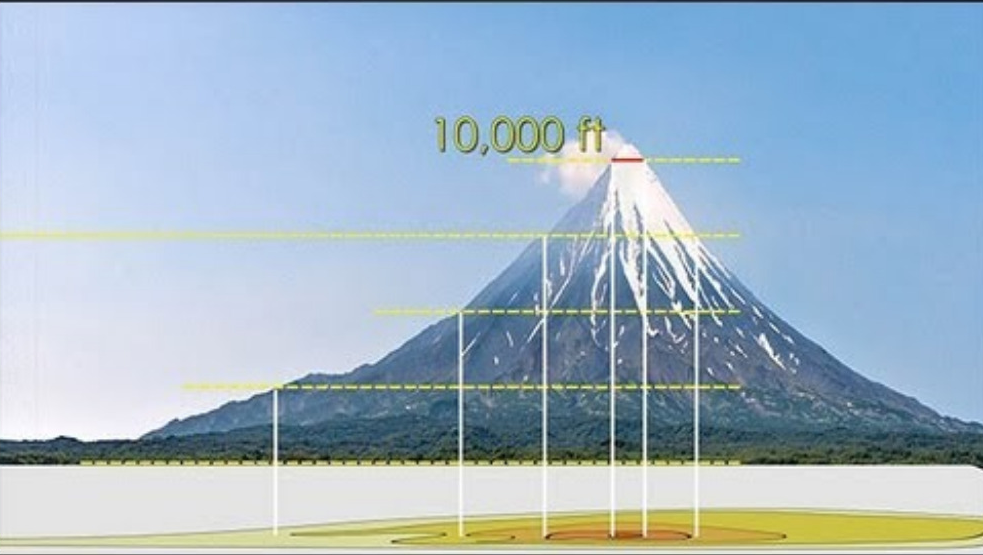
\includegraphics[width=0.62\textwidth]{images/mountain-contours.png}
\end{center}

%==========================================================
\section*{2. How to Draw an Isoline}

\begin{enumerate}[leftmargin=*,itemsep=6pt]
  \item Connect dots of \blk[3cm]{equal value}, using the interval stated in the directions.
  \item Where the exact number is not printed, \blk[2.5cm]{estimate} where it would fall between a point of higher value and a point of lower value.
  \item Bring every isoline all the way to the \blk[3cm]{edge of the field}.
\end{enumerate}

\textbf{Rules isolines never break:}

\begin{multicols}{2}
\begin{itemize}[leftmargin=*,itemsep=4pt]
  \item Isolines never \blk[2cm]{cross} each other.
  \item Isolines never split or branch.
  \item Isolines close into loops or run off the map edge.
  \item Values change \textbf{in order} --- no skipping.
  \item Lines close together $=$ value changing \blk[2cm]{quickly}.
  \item Lines far apart $=$ value changing \blk[2cm]{slowly}.
\end{itemize}
\end{multicols}

\subsection*{Practice: elevation field (contour interval = 10 ft)}

Draw contour lines at 40, 50, 60, 70, and 80 feet. Label each line and carry it to the edge of the box.

\begin{center}
\begin{tikzpicture}[x=2.0cm,y=1.5cm]
  \def\vals{
    {42,48,55,61,58,51},
    {47,56,68,72,65,55},
    {52,63,78,85,71,58},
    {49,58,70,76,66,54},
    {44,51,59,63,57,48},
    {38,43,48,52,47,41}}
  \foreach \row [count=\r from 0] in \vals {
    \foreach \v [count=\c from 0] in \row {
      \fill (\c,-\r) circle (1.3pt);
      \node[anchor=south west,font=\small,inner sep=1.5pt] at (\c,-\r) {\v};
    }
  }
  \draw[thick] (-0.35,0.6) rectangle (5.55,-7.85);
  \node[anchor=north west,font=\small\itshape] at (-0.35,-7.95) {Elevation (feet)};
\end{tikzpicture}
\end{center}

\teachernote{The 80-ft line is a small closed loop around the 85 value near the center; the 40-ft line only appears along the bottom edge. Watch for students who connect \textit{nearest dots} instead of \textit{equal values} --- have them label the two dots they are interpolating between before they draw.}

%==========================================================
\newpage
\section*{3. Map Scale and Direction}

\term{Map scale:} a ratio of the distance between two places on a map and the \blk[4cm]{actual distance} on Earth's surface.

\term{Cardinal directions:} \blk[1.8cm]{north}, \blk[1.8cm]{south}, \blk[1.8cm]{east}, \blk[1.8cm]{west}, and any combination of these (NE, SW, \dots).

\begin{center}
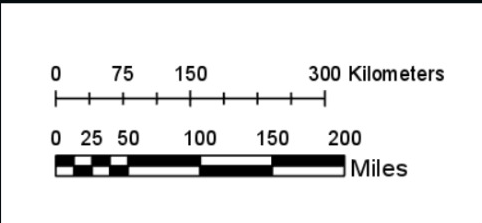
\includegraphics[width=0.42\textwidth]{images/map-scale.png}
\hspace{0.5cm}
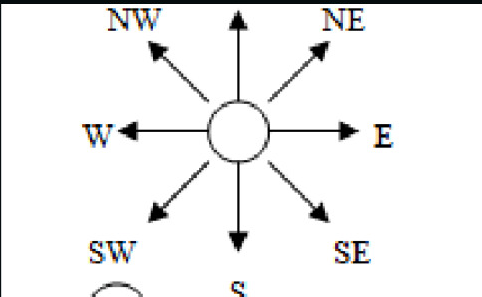
\includegraphics[width=0.26\textwidth]{images/compass-rose.png}
\end{center}

%==========================================================
\section*{4. Constructing a Profile}

A \term{profile} is a \blk[3.5cm]{side view} of the land along a line drawn on the map.

\begin{enumerate}[leftmargin=*,itemsep=6pt]
  \item Line the edge of a piece of \blk[3cm]{scrap paper} up with the two points on your map.
  \item Mark the two endpoints, plus every \blk[3cm]{contour line} that falls between them.
  \item Write the \blk[2cm]{value} of every mark.
  \item Line the paper edge up with the \blk[2cm]{x-axis} of your graph (first point at the origin) and plot each elevation against the \blk[2cm]{y-axis}.
  \item Connect your points with a \blk[3cm]{smooth curve}.
\end{enumerate}

\begin{callout}
\textbf{Round out the tops of your peaks and the bottoms of your valleys.} The land keeps rising past the last contour line you crossed, so the hilltop is rounded --- not a sharp point. \textbf{Straight lines and sharp peaks receive no credit.}
\end{callout}

\begin{center}
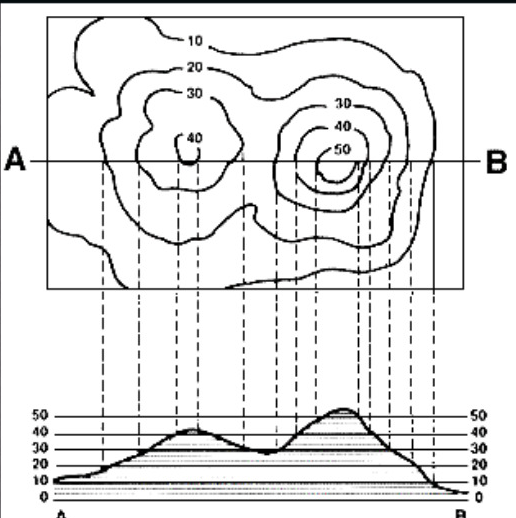
\includegraphics[width=0.38\textwidth]{images/profile-ab.png}
\end{center}

\subsection*{Practice: plot the profile}

Elevations were read along line A--B and recorded below. Plot each point, then connect them with a smooth, rounded curve.

\begin{center}
\small
\begin{tabular}{|c|c|c|c|c|c|c|c|c|c|c|c|}
\hline
\textbf{Point} & A & 2 & 3 & 4 & 5 & 6 & 7 & 8 & 9 & 10 & B \\ \hline
\textbf{Elev. (ft)} & 20 & 30 & 40 & 40 & 30 & 20 & 30 & 40 & 50 & 40 & 30 \\ \hline
\end{tabular}
\end{center}

\begin{center}
\begin{tikzpicture}[x=1.3cm,y=0.09cm]
  \draw[gray!45] (0,0) grid[xstep=1.3cm,ystep=0.09cm] (10,60);
  \foreach \y in {0,10,20,30,40,50,60} {
    \draw[gray!70] (0,\y) -- (10,\y);
    \node[anchor=east,font=\small] at (-0.08,\y) {\y};
  }
  \foreach \x in {0,1,2,3,4,5,6,7,8,9,10} \draw[gray!70] (\x,0) -- (\x,60);
  \draw[thick] (0,0) rectangle (10,60);
  \node[anchor=north,font=\small] at (0,-1) {A};
  \node[anchor=north,font=\small] at (10,-1) {B};
  \foreach \x [count=\i from 2] in {1,2,3,4,5,6,7,8,9} \node[anchor=north,font=\small] at (\x,-1) {\i};
  \node[rotate=90,anchor=south,font=\small] at (-0.75,30) {Elevation (ft)};
  \ifprintanswers
    \draw[keyblue,very thick,smooth]
      plot coordinates {(0,20) (1,30) (2,40) (3,40) (4,30) (5,20) (6,30) (7,40) (8,50) (9,40) (10,30)};
    \foreach \p in {(0,20),(1,30),(2,40),(3,40),(4,30),(5,20),(6,30),(7,40),(8,50),(9,40),(10,30)}
      \fill[keyblue] \p circle (2.2pt);
  \fi
\end{tikzpicture}
\end{center}

\teachernote{The key shows the plotted points connected point-to-point. Students should smooth the curve and round the two hilltops \textit{above} 40 ft and 50 ft respectively, and round the low point near point 6 --- the exact values between marks are unknown, which is the whole reason the curve is drawn smooth.}

%==========================================================
\newpage
\section*{5. Contour Lines and Streams}

\begin{itemize}[leftmargin=*,itemsep=4pt]
  \item Contour lines \blk[2cm]{bend} where they cross a stream.
  \item The bend forms a V that points \blk[2.5cm]{upstream} (uphill).
  \item Water flows \blk[2.5cm]{downhill}, so the stream flows in the \textbf{opposite} direction from the V.
  \item Streams run from \blk[2cm]{high} elevation toward \blk[2cm]{low} elevation.
\end{itemize}

\begin{center}
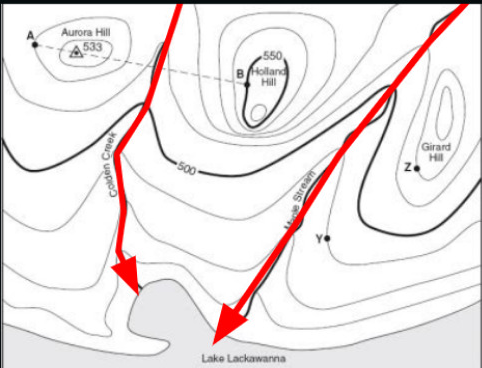
\includegraphics[width=0.60\textwidth]{images/stream-contours.png}
\end{center}

\begin{questions}

\question[2] On the map above, in which compass direction does Coldan Creek flow? Explain how the contour lines tell you.
\ifprintanswers
  \par\textcolor{keyblue}{\textbf{South (toward Lake Lackawanna).} The Vs in the contour lines point north --- upstream --- and the contour values decrease toward the lake, so the water flows south, from high elevation to low.}
\else
  \fillwithlines{0.9in}
\fi

\end{questions}

%==========================================================
\section*{6. Gradient}

Gradient tells you how \blk[2.5cm]{steep} a slope is. The equation is on page \blk[1cm]{1} of the ESRT:

\begin{callout}
\[ \text{Gradient} = \frac{\text{change in field value}}{\text{distance}} \]
\end{callout}

The closer the isolines are together in a given distance, the \blk[2cm]{larger} the gradient.

\textbf{Worked example.} Point A is at 123 feet. Point B is at 20 feet. The points are 2 miles apart.

\[ \text{Gradient} = \frac{123\ \text{ft} - 20\ \text{ft}}{2\ \text{mi}} = \frac{\blk[1.6cm]{103}\ \text{ft}}{2\ \text{mi}} = \blk[2cm]{51.5}\ \text{ft/mi} \]

\begin{center}\textbf{DON'T FORGET UNITS!}\end{center}

\teachernote{Require all three steps every time --- equation, substitution with units, answer with units. Regents rubrics award credit for the setup even when the arithmetic slips.}

\begin{questions}

\question[3] Point A has an elevation of 260 feet. Point B has an elevation of 10 feet. The points are 3 miles apart. Calculate the gradient. Show the equation, your substitution, and the units.
\ifprintanswers
  \par\textcolor{keyblue}{$\text{Gradient} = \dfrac{\text{change in field value}}{\text{distance}} = \dfrac{260\ \text{ft} - 10\ \text{ft}}{3\ \text{mi}} = \dfrac{250\ \text{ft}}{3\ \text{mi}} = \mathbf{83.3\ \text{ft/mi}}$}
\else
  \fillwithlines{1.1in}
\fi

\question[3] A hilltop is 550 meters above sea level. A stream at the base of the hill is 250 meters above sea level. The horizontal distance between them is 1.5 kilometers. Calculate the gradient.
\ifprintanswers
  \par\textcolor{keyblue}{$\dfrac{550\ \text{m} - 250\ \text{m}}{1.5\ \text{km}} = \dfrac{300\ \text{m}}{1.5\ \text{km}} = \mathbf{200\ \text{m/km}}$}
\else
  \fillwithlines{1.1in}
\fi

\question[3] On a weather map, one station reports 82\,$^\circ$F and another reports 58\,$^\circ$F. The stations are 4 kilometers apart. Calculate the temperature gradient between them.
\ifprintanswers
  \par\textcolor{keyblue}{$\dfrac{82\,^\circ\text{F} - 58\,^\circ\text{F}}{4\ \text{km}} = \dfrac{24\,^\circ\text{F}}{4\ \text{km}} = \mathbf{6\,^\circ\text{F/km}}$ --- gradient works on \textit{any} field, not just elevation.}
\else
  \fillwithlines{1.1in}
\fi

\question[2] Two trails climb the same hill. Trail X crosses contour lines that are crowded close together; trail Y crosses contour lines that are widely spaced. Which trail is steeper, and how do you know?
\ifprintanswers
  \par\textcolor{keyblue}{\textbf{Trail X.} Crowded contours mean a large change in elevation over a short distance, which is a large gradient --- a steeper slope.}
\else
  \fillwithlines{0.9in}
\fi

\end{questions}

%==========================================================
\section*{7. Exit Ticket}

\begin{questions}

\question[1] What does a contour line connect?
\ifprintanswers
  \par\textcolor{keyblue}{Points of equal elevation.}
\else
  \fillwithlines{0.5in}
\fi

\question[1] A stream crosses a contour line. Which direction does the V point?
\ifprintanswers
  \par\textcolor{keyblue}{Upstream --- toward higher elevation, opposite the direction the water flows.}
\else
  \fillwithlines{0.5in}
\fi

\question[1] Why must the top of a hill on a profile be drawn rounded instead of pointed?
\ifprintanswers
  \par\textcolor{keyblue}{The land continues to rise above the highest contour line crossed, but the exact summit elevation is unknown, so the curve is rounded through that unknown space rather than drawn to a sharp point.}
\else
  \fillwithlines{0.6in}
\fi

\end{questions}

\end{document}
"
%\printanswers  % <-- or just uncomment this line for the answer key

\usepackage[margin=0.85in,top=1.0in,headsep=0.25in]{geometry}
\usepackage{graphicx}
\usepackage{amsmath}
\usepackage{xcolor}
\usepackage{tikz}
\usepackage{enumitem}
\usepackage{multicol}
\usepackage{tcolorbox}

\definecolor{keyblue}{RGB}{0,70,190}
\definecolor{accent}{RGB}{29,107,132}
\definecolor{shade}{RGB}{234,243,246}

\setlength{\parindent}{0pt}
\setlength{\parskip}{4pt}

% ---------- fill-in-the-blank macro ----------
% \blk{answer} or \blk[width]{answer}
\newcommand{\blk}[2][3.2cm]{%
  \ifprintanswers
    \underline{\textcolor{keyblue}{\textbf{#2}}}%
  \else
    \underline{\hspace{#1}}%
  \fi}

% teacher-only note
\newcommand{\teachernote}[1]{\ifprintanswers\par\textcolor{accent}{\textit{Teacher note: #1}}\par\fi}

\newcommand{\term}[1]{\textbf{\textcolor{accent}{#1}}}

\newtcolorbox{callout}{colback=shade,colframe=accent,boxrule=0.8pt,left=8pt,right=8pt,top=6pt,bottom=6pt,arc=2pt}

% ---------- header ----------
\pagestyle{headandfoot}
\header{\textbf{Topographic Mapping --- Guided Notes}}{}{%
  \ifprintanswers\textcolor{keyblue}{\textbf{ANSWER KEY}}\else Name: \underline{\hspace{4cm}}\fi}
\footer{}{Page \thepage\ of \numpages}{}
\runningheadrule
\runningfootrule

\begin{document}

\ifprintanswers\else
{\small Period: \underline{\hspace{2cm}} \hfill Date: \underline{\hspace{3.5cm}}}
\vspace{6pt}
\fi

\begin{callout}
\textbf{Objective:} Use isolines to represent field data, construct a topographic profile from a contour map, and calculate gradient using the ESRT equation.
\end{callout}

%==========================================================
\section*{1. Mapping the Earth: Terms}

A \term{field} is any region of space that has a measurable value of a given quantity at \blk[3cm]{every point}.

An \term{isoline} is a line that connects points of \blk[3.5cm]{equal value}.

\vspace{4pt}
Fill in the table:

\begin{center}
\renewcommand{\arraystretch}{1.7}
\begin{tabular}{|p{3.2cm}|p{5.5cm}|p{4.5cm}|}
\hline
\textbf{Type of isoline} & \textbf{Connects points of equal\dots} & \textbf{Where you see it} \\ \hline
Isotherm & \blk[3.5cm]{temperature} & Weather map \\ \hline
Isobar & \blk[3.5cm]{pressure} & Weather map \\ \hline
Contour line & \blk[3.5cm]{elevation} & Topographic map \\ \hline
\end{tabular}
\end{center}

\teachernote{Point out the prefix \textit{iso-} = equal. Students who learn the prefix can decode any isoline question on the Regents exam, including ones they have never seen (isoseismal, isohyet).}

\vspace{4pt}
A topographic map shows a \blk[2.5cm]{3-D} landscape on a \blk[2.5cm]{2-D} sheet of paper. Each contour line traces one elevation all the way around the landform.

\begin{center}
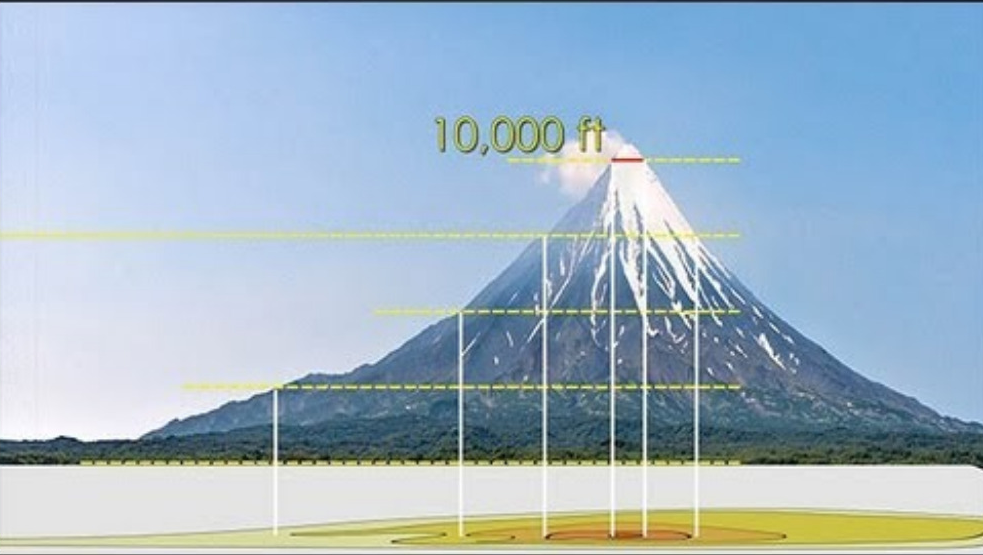
\includegraphics[width=0.62\textwidth]{images/mountain-contours.png}
\end{center}

%==========================================================
\section*{2. How to Draw an Isoline}

\begin{enumerate}[leftmargin=*,itemsep=6pt]
  \item Connect dots of \blk[3cm]{equal value}, using the interval stated in the directions.
  \item Where the exact number is not printed, \blk[2.5cm]{estimate} where it would fall between a point of higher value and a point of lower value.
  \item Bring every isoline all the way to the \blk[3cm]{edge of the field}.
\end{enumerate}

\textbf{Rules isolines never break:}

\begin{multicols}{2}
\begin{itemize}[leftmargin=*,itemsep=4pt]
  \item Isolines never \blk[2cm]{cross} each other.
  \item Isolines never split or branch.
  \item Isolines close into loops or run off the map edge.
  \item Values change \textbf{in order} --- no skipping.
  \item Lines close together $=$ value changing \blk[2cm]{quickly}.
  \item Lines far apart $=$ value changing \blk[2cm]{slowly}.
\end{itemize}
\end{multicols}

\subsection*{Practice: elevation field (contour interval = 10 ft)}

Draw contour lines at 40, 50, 60, 70, and 80 feet. Label each line and carry it to the edge of the box.

\begin{center}
\begin{tikzpicture}[x=2.0cm,y=1.5cm]
  \def\vals{
    {42,48,55,61,58,51},
    {47,56,68,72,65,55},
    {52,63,78,85,71,58},
    {49,58,70,76,66,54},
    {44,51,59,63,57,48},
    {38,43,48,52,47,41}}
  \foreach \row [count=\r from 0] in \vals {
    \foreach \v [count=\c from 0] in \row {
      \fill (\c,-\r) circle (1.3pt);
      \node[anchor=south west,font=\small,inner sep=1.5pt] at (\c,-\r) {\v};
    }
  }
  \draw[thick] (-0.35,0.6) rectangle (5.55,-7.85);
  \node[anchor=north west,font=\small\itshape] at (-0.35,-7.95) {Elevation (feet)};
\end{tikzpicture}
\end{center}

\teachernote{The 80-ft line is a small closed loop around the 85 value near the center; the 40-ft line only appears along the bottom edge. Watch for students who connect \textit{nearest dots} instead of \textit{equal values} --- have them label the two dots they are interpolating between before they draw.}

%==========================================================
\newpage
\section*{3. Map Scale and Direction}

\term{Map scale:} a ratio of the distance between two places on a map and the \blk[4cm]{actual distance} on Earth's surface.

\term{Cardinal directions:} \blk[1.8cm]{north}, \blk[1.8cm]{south}, \blk[1.8cm]{east}, \blk[1.8cm]{west}, and any combination of these (NE, SW, \dots).

\begin{center}
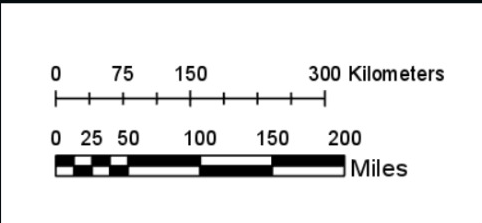
\includegraphics[width=0.42\textwidth]{images/map-scale.png}
\hspace{0.5cm}
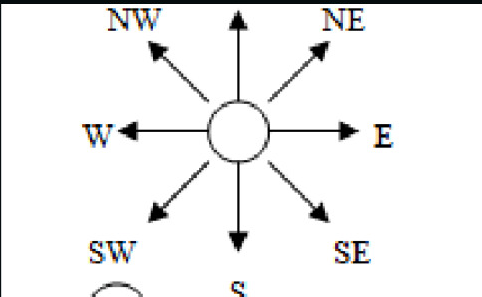
\includegraphics[width=0.26\textwidth]{images/compass-rose.png}
\end{center}

%==========================================================
\section*{4. Constructing a Profile}

A \term{profile} is a \blk[3.5cm]{side view} of the land along a line drawn on the map.

\begin{enumerate}[leftmargin=*,itemsep=6pt]
  \item Line the edge of a piece of \blk[3cm]{scrap paper} up with the two points on your map.
  \item Mark the two endpoints, plus every \blk[3cm]{contour line} that falls between them.
  \item Write the \blk[2cm]{value} of every mark.
  \item Line the paper edge up with the \blk[2cm]{x-axis} of your graph (first point at the origin) and plot each elevation against the \blk[2cm]{y-axis}.
  \item Connect your points with a \blk[3cm]{smooth curve}.
\end{enumerate}

\begin{callout}
\textbf{Round out the tops of your peaks and the bottoms of your valleys.} The land keeps rising past the last contour line you crossed, so the hilltop is rounded --- not a sharp point. \textbf{Straight lines and sharp peaks receive no credit.}
\end{callout}

\begin{center}
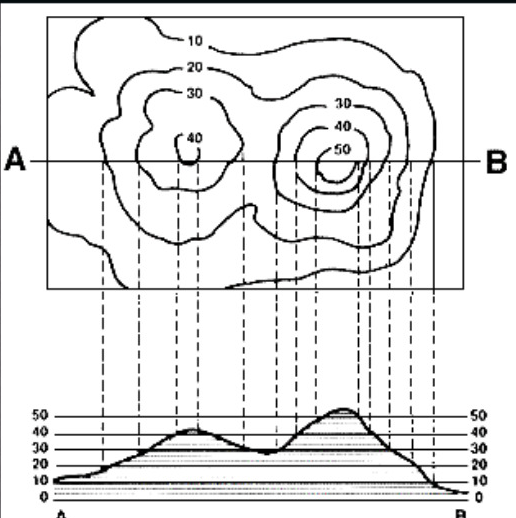
\includegraphics[width=0.38\textwidth]{images/profile-ab.png}
\end{center}

\subsection*{Practice: plot the profile}

Elevations were read along line A--B and recorded below. Plot each point, then connect them with a smooth, rounded curve.

\begin{center}
\small
\begin{tabular}{|c|c|c|c|c|c|c|c|c|c|c|c|}
\hline
\textbf{Point} & A & 2 & 3 & 4 & 5 & 6 & 7 & 8 & 9 & 10 & B \\ \hline
\textbf{Elev. (ft)} & 20 & 30 & 40 & 40 & 30 & 20 & 30 & 40 & 50 & 40 & 30 \\ \hline
\end{tabular}
\end{center}

\begin{center}
\begin{tikzpicture}[x=1.3cm,y=0.09cm]
  \draw[gray!45] (0,0) grid[xstep=1.3cm,ystep=0.09cm] (10,60);
  \foreach \y in {0,10,20,30,40,50,60} {
    \draw[gray!70] (0,\y) -- (10,\y);
    \node[anchor=east,font=\small] at (-0.08,\y) {\y};
  }
  \foreach \x in {0,1,2,3,4,5,6,7,8,9,10} \draw[gray!70] (\x,0) -- (\x,60);
  \draw[thick] (0,0) rectangle (10,60);
  \node[anchor=north,font=\small] at (0,-1) {A};
  \node[anchor=north,font=\small] at (10,-1) {B};
  \foreach \x [count=\i from 2] in {1,2,3,4,5,6,7,8,9} \node[anchor=north,font=\small] at (\x,-1) {\i};
  \node[rotate=90,anchor=south,font=\small] at (-0.75,30) {Elevation (ft)};
  \ifprintanswers
    \draw[keyblue,very thick,smooth]
      plot coordinates {(0,20) (1,30) (2,40) (3,40) (4,30) (5,20) (6,30) (7,40) (8,50) (9,40) (10,30)};
    \foreach \p in {(0,20),(1,30),(2,40),(3,40),(4,30),(5,20),(6,30),(7,40),(8,50),(9,40),(10,30)}
      \fill[keyblue] \p circle (2.2pt);
  \fi
\end{tikzpicture}
\end{center}

\teachernote{The key shows the plotted points connected point-to-point. Students should smooth the curve and round the two hilltops \textit{above} 40 ft and 50 ft respectively, and round the low point near point 6 --- the exact values between marks are unknown, which is the whole reason the curve is drawn smooth.}

%==========================================================
\newpage
\section*{5. Contour Lines and Streams}

\begin{itemize}[leftmargin=*,itemsep=4pt]
  \item Contour lines \blk[2cm]{bend} where they cross a stream.
  \item The bend forms a V that points \blk[2.5cm]{upstream} (uphill).
  \item Water flows \blk[2.5cm]{downhill}, so the stream flows in the \textbf{opposite} direction from the V.
  \item Streams run from \blk[2cm]{high} elevation toward \blk[2cm]{low} elevation.
\end{itemize}

\begin{center}
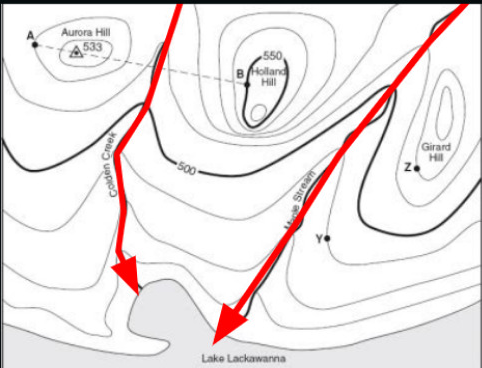
\includegraphics[width=0.60\textwidth]{images/stream-contours.png}
\end{center}

\begin{questions}

\question[2] On the map above, in which compass direction does Coldan Creek flow? Explain how the contour lines tell you.
\ifprintanswers
  \par\textcolor{keyblue}{\textbf{South (toward Lake Lackawanna).} The Vs in the contour lines point north --- upstream --- and the contour values decrease toward the lake, so the water flows south, from high elevation to low.}
\else
  \fillwithlines{0.9in}
\fi

\end{questions}

%==========================================================
\section*{6. Gradient}

Gradient tells you how \blk[2.5cm]{steep} a slope is. The equation is on page \blk[1cm]{1} of the ESRT:

\begin{callout}
\[ \text{Gradient} = \frac{\text{change in field value}}{\text{distance}} \]
\end{callout}

The closer the isolines are together in a given distance, the \blk[2cm]{larger} the gradient.

\textbf{Worked example.} Point A is at 123 feet. Point B is at 20 feet. The points are 2 miles apart.

\[ \text{Gradient} = \frac{123\ \text{ft} - 20\ \text{ft}}{2\ \text{mi}} = \frac{\blk[1.6cm]{103}\ \text{ft}}{2\ \text{mi}} = \blk[2cm]{51.5}\ \text{ft/mi} \]

\begin{center}\textbf{DON'T FORGET UNITS!}\end{center}

\teachernote{Require all three steps every time --- equation, substitution with units, answer with units. Regents rubrics award credit for the setup even when the arithmetic slips.}

\begin{questions}

\question[3] Point A has an elevation of 260 feet. Point B has an elevation of 10 feet. The points are 3 miles apart. Calculate the gradient. Show the equation, your substitution, and the units.
\ifprintanswers
  \par\textcolor{keyblue}{$\text{Gradient} = \dfrac{\text{change in field value}}{\text{distance}} = \dfrac{260\ \text{ft} - 10\ \text{ft}}{3\ \text{mi}} = \dfrac{250\ \text{ft}}{3\ \text{mi}} = \mathbf{83.3\ \text{ft/mi}}$}
\else
  \fillwithlines{1.1in}
\fi

\question[3] A hilltop is 550 meters above sea level. A stream at the base of the hill is 250 meters above sea level. The horizontal distance between them is 1.5 kilometers. Calculate the gradient.
\ifprintanswers
  \par\textcolor{keyblue}{$\dfrac{550\ \text{m} - 250\ \text{m}}{1.5\ \text{km}} = \dfrac{300\ \text{m}}{1.5\ \text{km}} = \mathbf{200\ \text{m/km}}$}
\else
  \fillwithlines{1.1in}
\fi

\question[3] On a weather map, one station reports 82\,$^\circ$F and another reports 58\,$^\circ$F. The stations are 4 kilometers apart. Calculate the temperature gradient between them.
\ifprintanswers
  \par\textcolor{keyblue}{$\dfrac{82\,^\circ\text{F} - 58\,^\circ\text{F}}{4\ \text{km}} = \dfrac{24\,^\circ\text{F}}{4\ \text{km}} = \mathbf{6\,^\circ\text{F/km}}$ --- gradient works on \textit{any} field, not just elevation.}
\else
  \fillwithlines{1.1in}
\fi

\question[2] Two trails climb the same hill. Trail X crosses contour lines that are crowded close together; trail Y crosses contour lines that are widely spaced. Which trail is steeper, and how do you know?
\ifprintanswers
  \par\textcolor{keyblue}{\textbf{Trail X.} Crowded contours mean a large change in elevation over a short distance, which is a large gradient --- a steeper slope.}
\else
  \fillwithlines{0.9in}
\fi

\end{questions}

%==========================================================
\section*{7. Exit Ticket}

\begin{questions}

\question[1] What does a contour line connect?
\ifprintanswers
  \par\textcolor{keyblue}{Points of equal elevation.}
\else
  \fillwithlines{0.5in}
\fi

\question[1] A stream crosses a contour line. Which direction does the V point?
\ifprintanswers
  \par\textcolor{keyblue}{Upstream --- toward higher elevation, opposite the direction the water flows.}
\else
  \fillwithlines{0.5in}
\fi

\question[1] Why must the top of a hill on a profile be drawn rounded instead of pointed?
\ifprintanswers
  \par\textcolor{keyblue}{The land continues to rise above the highest contour line crossed, but the exact summit elevation is unknown, so the curve is rounded through that unknown space rather than drawn to a sharp point.}
\else
  \fillwithlines{0.6in}
\fi

\end{questions}

\end{document}
"
%\printanswers  % <-- or just uncomment this line for the answer key

\usepackage[margin=0.85in,top=1.0in,headsep=0.25in]{geometry}
\usepackage{graphicx}
\usepackage{amsmath}
\usepackage{xcolor}
\usepackage{tikz}
\usepackage{enumitem}
\usepackage{multicol}
\usepackage{tcolorbox}

\definecolor{keyblue}{RGB}{0,70,190}
\definecolor{accent}{RGB}{29,107,132}
\definecolor{shade}{RGB}{234,243,246}

\setlength{\parindent}{0pt}
\setlength{\parskip}{4pt}

% ---------- fill-in-the-blank macro ----------
% \blk{answer} or \blk[width]{answer}
\newcommand{\blk}[2][3.2cm]{%
  \ifprintanswers
    \underline{\textcolor{keyblue}{\textbf{#2}}}%
  \else
    \underline{\hspace{#1}}%
  \fi}

% teacher-only note
\newcommand{\teachernote}[1]{\ifprintanswers\par\textcolor{accent}{\textit{Teacher note: #1}}\par\fi}

\newcommand{\term}[1]{\textbf{\textcolor{accent}{#1}}}

\newtcolorbox{callout}{colback=shade,colframe=accent,boxrule=0.8pt,left=8pt,right=8pt,top=6pt,bottom=6pt,arc=2pt}

% ---------- header ----------
\pagestyle{headandfoot}
\header{\textbf{Topographic Mapping --- Guided Notes}}{}{%
  \ifprintanswers\textcolor{keyblue}{\textbf{ANSWER KEY}}\else Name: \underline{\hspace{4cm}}\fi}
\footer{}{Page \thepage\ of \numpages}{}
\runningheadrule
\runningfootrule

\begin{document}

\ifprintanswers\else
{\small Period: \underline{\hspace{2cm}} \hfill Date: \underline{\hspace{3.5cm}}}
\vspace{6pt}
\fi

\begin{callout}
\textbf{Objective:} Use isolines to represent field data, construct a topographic profile from a contour map, and calculate gradient using the ESRT equation.
\end{callout}

%==========================================================
\section*{1. Mapping the Earth: Terms}

A \term{field} is any region of space that has a measurable value of a given quantity at \blk[3cm]{every point}.

An \term{isoline} is a line that connects points of \blk[3.5cm]{equal value}.

\vspace{4pt}
Fill in the table:

\begin{center}
\renewcommand{\arraystretch}{1.7}
\begin{tabular}{|p{3.2cm}|p{5.5cm}|p{4.5cm}|}
\hline
\textbf{Type of isoline} & \textbf{Connects points of equal\dots} & \textbf{Where you see it} \\ \hline
Isotherm & \blk[3.5cm]{temperature} & Weather map \\ \hline
Isobar & \blk[3.5cm]{pressure} & Weather map \\ \hline
Contour line & \blk[3.5cm]{elevation} & Topographic map \\ \hline
\end{tabular}
\end{center}

\teachernote{Point out the prefix \textit{iso-} = equal. Students who learn the prefix can decode any isoline question on the Regents exam, including ones they have never seen (isoseismal, isohyet).}

\vspace{4pt}
A topographic map shows a \blk[2.5cm]{3-D} landscape on a \blk[2.5cm]{2-D} sheet of paper. Each contour line traces one elevation all the way around the landform.

\begin{center}
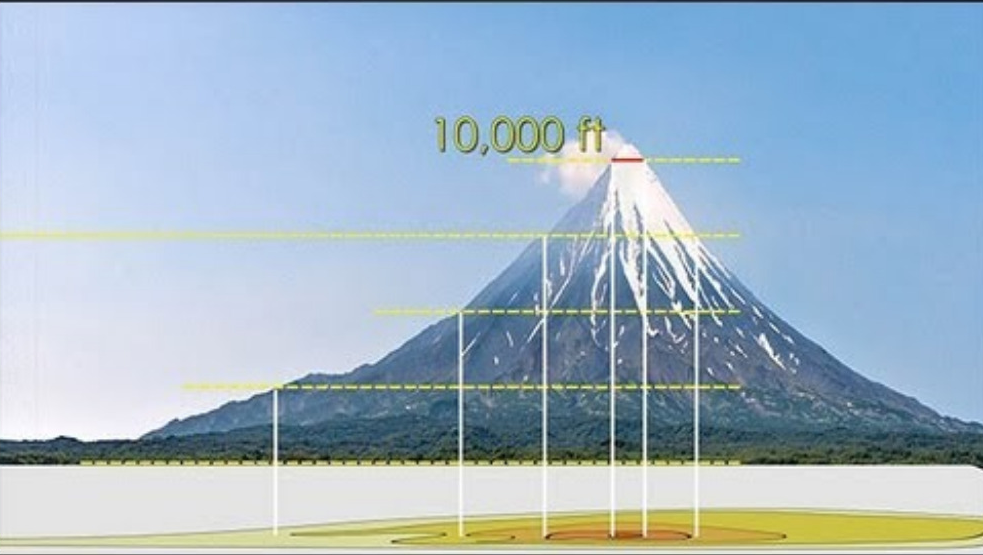
\includegraphics[width=0.62\textwidth]{images/mountain-contours.png}
\end{center}

%==========================================================
\section*{2. How to Draw an Isoline}

\begin{enumerate}[leftmargin=*,itemsep=6pt]
  \item Connect dots of \blk[3cm]{equal value}, using the interval stated in the directions.
  \item Where the exact number is not printed, \blk[2.5cm]{estimate} where it would fall between a point of higher value and a point of lower value.
  \item Bring every isoline all the way to the \blk[3cm]{edge of the field}.
\end{enumerate}

\textbf{Rules isolines never break:}

\begin{multicols}{2}
\begin{itemize}[leftmargin=*,itemsep=4pt]
  \item Isolines never \blk[2cm]{cross} each other.
  \item Isolines never split or branch.
  \item Isolines close into loops or run off the map edge.
  \item Values change \textbf{in order} --- no skipping.
  \item Lines close together $=$ value changing \blk[2cm]{quickly}.
  \item Lines far apart $=$ value changing \blk[2cm]{slowly}.
\end{itemize}
\end{multicols}

\subsection*{Practice: elevation field (contour interval = 10 ft)}

Draw contour lines at 40, 50, 60, 70, and 80 feet. Label each line and carry it to the edge of the box.

\begin{center}
\begin{tikzpicture}[x=2.0cm,y=1.5cm]
  \def\vals{
    {42,48,55,61,58,51},
    {47,56,68,72,65,55},
    {52,63,78,85,71,58},
    {49,58,70,76,66,54},
    {44,51,59,63,57,48},
    {38,43,48,52,47,41}}
  \foreach \row [count=\r from 0] in \vals {
    \foreach \v [count=\c from 0] in \row {
      \fill (\c,-\r) circle (1.3pt);
      \node[anchor=south west,font=\small,inner sep=1.5pt] at (\c,-\r) {\v};
    }
  }
  \draw[thick] (-0.35,0.6) rectangle (5.55,-7.85);
  \node[anchor=north west,font=\small\itshape] at (-0.35,-7.95) {Elevation (feet)};
\end{tikzpicture}
\end{center}

\teachernote{The 80-ft line is a small closed loop around the 85 value near the center; the 40-ft line only appears along the bottom edge. Watch for students who connect \textit{nearest dots} instead of \textit{equal values} --- have them label the two dots they are interpolating between before they draw.}

%==========================================================
\newpage
\section*{3. Map Scale and Direction}

\term{Map scale:} a ratio of the distance between two places on a map and the \blk[4cm]{actual distance} on Earth's surface.

\term{Cardinal directions:} \blk[1.8cm]{north}, \blk[1.8cm]{south}, \blk[1.8cm]{east}, \blk[1.8cm]{west}, and any combination of these (NE, SW, \dots).

\begin{center}
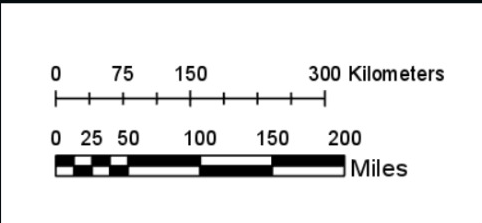
\includegraphics[width=0.42\textwidth]{images/map-scale.png}
\hspace{0.5cm}
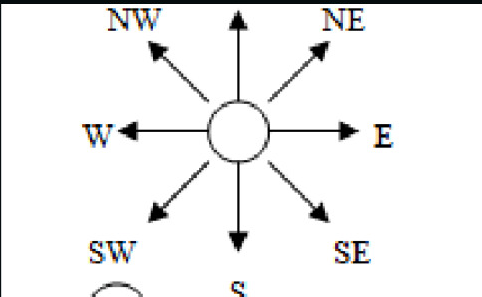
\includegraphics[width=0.26\textwidth]{images/compass-rose.png}
\end{center}

%==========================================================
\section*{4. Constructing a Profile}

A \term{profile} is a \blk[3.5cm]{side view} of the land along a line drawn on the map.

\begin{enumerate}[leftmargin=*,itemsep=6pt]
  \item Line the edge of a piece of \blk[3cm]{scrap paper} up with the two points on your map.
  \item Mark the two endpoints, plus every \blk[3cm]{contour line} that falls between them.
  \item Write the \blk[2cm]{value} of every mark.
  \item Line the paper edge up with the \blk[2cm]{x-axis} of your graph (first point at the origin) and plot each elevation against the \blk[2cm]{y-axis}.
  \item Connect your points with a \blk[3cm]{smooth curve}.
\end{enumerate}

\begin{callout}
\textbf{Round out the tops of your peaks and the bottoms of your valleys.} The land keeps rising past the last contour line you crossed, so the hilltop is rounded --- not a sharp point. \textbf{Straight lines and sharp peaks receive no credit.}
\end{callout}

\begin{center}
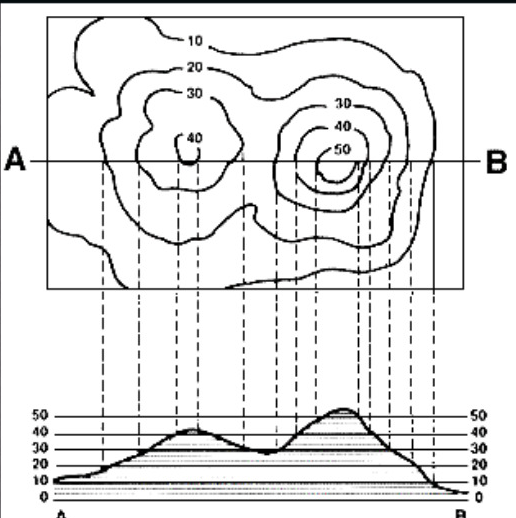
\includegraphics[width=0.38\textwidth]{images/profile-ab.png}
\end{center}

\subsection*{Practice: plot the profile}

Elevations were read along line A--B and recorded below. Plot each point, then connect them with a smooth, rounded curve.

\begin{center}
\small
\begin{tabular}{|c|c|c|c|c|c|c|c|c|c|c|c|}
\hline
\textbf{Point} & A & 2 & 3 & 4 & 5 & 6 & 7 & 8 & 9 & 10 & B \\ \hline
\textbf{Elev. (ft)} & 20 & 30 & 40 & 40 & 30 & 20 & 30 & 40 & 50 & 40 & 30 \\ \hline
\end{tabular}
\end{center}

\begin{center}
\begin{tikzpicture}[x=1.3cm,y=0.09cm]
  \draw[gray!45] (0,0) grid[xstep=1.3cm,ystep=0.09cm] (10,60);
  \foreach \y in {0,10,20,30,40,50,60} {
    \draw[gray!70] (0,\y) -- (10,\y);
    \node[anchor=east,font=\small] at (-0.08,\y) {\y};
  }
  \foreach \x in {0,1,2,3,4,5,6,7,8,9,10} \draw[gray!70] (\x,0) -- (\x,60);
  \draw[thick] (0,0) rectangle (10,60);
  \node[anchor=north,font=\small] at (0,-1) {A};
  \node[anchor=north,font=\small] at (10,-1) {B};
  \foreach \x [count=\i from 2] in {1,2,3,4,5,6,7,8,9} \node[anchor=north,font=\small] at (\x,-1) {\i};
  \node[rotate=90,anchor=south,font=\small] at (-0.75,30) {Elevation (ft)};
  \ifprintanswers
    \draw[keyblue,very thick,smooth]
      plot coordinates {(0,20) (1,30) (2,40) (3,40) (4,30) (5,20) (6,30) (7,40) (8,50) (9,40) (10,30)};
    \foreach \p in {(0,20),(1,30),(2,40),(3,40),(4,30),(5,20),(6,30),(7,40),(8,50),(9,40),(10,30)}
      \fill[keyblue] \p circle (2.2pt);
  \fi
\end{tikzpicture}
\end{center}

\teachernote{The key shows the plotted points connected point-to-point. Students should smooth the curve and round the two hilltops \textit{above} 40 ft and 50 ft respectively, and round the low point near point 6 --- the exact values between marks are unknown, which is the whole reason the curve is drawn smooth.}

%==========================================================
\newpage
\section*{5. Contour Lines and Streams}

\begin{itemize}[leftmargin=*,itemsep=4pt]
  \item Contour lines \blk[2cm]{bend} where they cross a stream.
  \item The bend forms a V that points \blk[2.5cm]{upstream} (uphill).
  \item Water flows \blk[2.5cm]{downhill}, so the stream flows in the \textbf{opposite} direction from the V.
  \item Streams run from \blk[2cm]{high} elevation toward \blk[2cm]{low} elevation.
\end{itemize}

\begin{center}
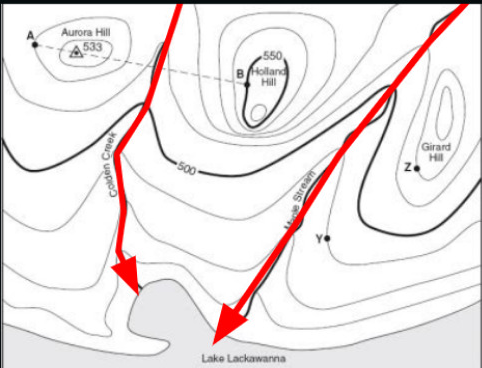
\includegraphics[width=0.60\textwidth]{images/stream-contours.png}
\end{center}

\begin{questions}

\question[2] On the map above, in which compass direction does Coldan Creek flow? Explain how the contour lines tell you.
\ifprintanswers
  \par\textcolor{keyblue}{\textbf{South (toward Lake Lackawanna).} The Vs in the contour lines point north --- upstream --- and the contour values decrease toward the lake, so the water flows south, from high elevation to low.}
\else
  \fillwithlines{0.9in}
\fi

\end{questions}

%==========================================================
\section*{6. Gradient}

Gradient tells you how \blk[2.5cm]{steep} a slope is. The equation is on page \blk[1cm]{1} of the ESRT:

\begin{callout}
\[ \text{Gradient} = \frac{\text{change in field value}}{\text{distance}} \]
\end{callout}

The closer the isolines are together in a given distance, the \blk[2cm]{larger} the gradient.

\textbf{Worked example.} Point A is at 123 feet. Point B is at 20 feet. The points are 2 miles apart.

\[ \text{Gradient} = \frac{123\ \text{ft} - 20\ \text{ft}}{2\ \text{mi}} = \frac{\blk[1.6cm]{103}\ \text{ft}}{2\ \text{mi}} = \blk[2cm]{51.5}\ \text{ft/mi} \]

\begin{center}\textbf{DON'T FORGET UNITS!}\end{center}

\teachernote{Require all three steps every time --- equation, substitution with units, answer with units. Regents rubrics award credit for the setup even when the arithmetic slips.}

\begin{questions}

\question[3] Point A has an elevation of 260 feet. Point B has an elevation of 10 feet. The points are 3 miles apart. Calculate the gradient. Show the equation, your substitution, and the units.
\ifprintanswers
  \par\textcolor{keyblue}{$\text{Gradient} = \dfrac{\text{change in field value}}{\text{distance}} = \dfrac{260\ \text{ft} - 10\ \text{ft}}{3\ \text{mi}} = \dfrac{250\ \text{ft}}{3\ \text{mi}} = \mathbf{83.3\ \text{ft/mi}}$}
\else
  \fillwithlines{1.1in}
\fi

\question[3] A hilltop is 550 meters above sea level. A stream at the base of the hill is 250 meters above sea level. The horizontal distance between them is 1.5 kilometers. Calculate the gradient.
\ifprintanswers
  \par\textcolor{keyblue}{$\dfrac{550\ \text{m} - 250\ \text{m}}{1.5\ \text{km}} = \dfrac{300\ \text{m}}{1.5\ \text{km}} = \mathbf{200\ \text{m/km}}$}
\else
  \fillwithlines{1.1in}
\fi

\question[3] On a weather map, one station reports 82\,$^\circ$F and another reports 58\,$^\circ$F. The stations are 4 kilometers apart. Calculate the temperature gradient between them.
\ifprintanswers
  \par\textcolor{keyblue}{$\dfrac{82\,^\circ\text{F} - 58\,^\circ\text{F}}{4\ \text{km}} = \dfrac{24\,^\circ\text{F}}{4\ \text{km}} = \mathbf{6\,^\circ\text{F/km}}$ --- gradient works on \textit{any} field, not just elevation.}
\else
  \fillwithlines{1.1in}
\fi

\question[2] Two trails climb the same hill. Trail X crosses contour lines that are crowded close together; trail Y crosses contour lines that are widely spaced. Which trail is steeper, and how do you know?
\ifprintanswers
  \par\textcolor{keyblue}{\textbf{Trail X.} Crowded contours mean a large change in elevation over a short distance, which is a large gradient --- a steeper slope.}
\else
  \fillwithlines{0.9in}
\fi

\end{questions}

%==========================================================
\section*{7. Exit Ticket}

\begin{questions}

\question[1] What does a contour line connect?
\ifprintanswers
  \par\textcolor{keyblue}{Points of equal elevation.}
\else
  \fillwithlines{0.5in}
\fi

\question[1] A stream crosses a contour line. Which direction does the V point?
\ifprintanswers
  \par\textcolor{keyblue}{Upstream --- toward higher elevation, opposite the direction the water flows.}
\else
  \fillwithlines{0.5in}
\fi

\question[1] Why must the top of a hill on a profile be drawn rounded instead of pointed?
\ifprintanswers
  \par\textcolor{keyblue}{The land continues to rise above the highest contour line crossed, but the exact summit elevation is unknown, so the curve is rounded through that unknown space rather than drawn to a sharp point.}
\else
  \fillwithlines{0.6in}
\fi

\end{questions}

\end{document}
